\chapter{Experiments}
\label{chapter:experiments}

\section{Full Lap Planning}

In this experiment we test the Hybrid A* and \gls{SEHS} algorithms as we described them in Section~\ref{sec:trajectory_planning_algorithms} on several different circuit maps. For each circuit, the algorithms should find a near time-optimal trajectory from a starting position through a series of waypoints until the last waypoint of the circuit is reached. We then compare the quality of the solutions, how much of the state space the algorithm had to explore before it found the solution, and how long it took to calculate the result on the testing computer.

\subsection{Test Setup}

Both Hybrid A* and \gls*{SEHS} are dependent on the level of discretization. The finer the discretization is, the closer the results are to the optimal solution. At the same time, the size of the searched state space increases. In order to compare our implementation of the two algorithms, we ran them with several different combinations parameter values.

The heading angle ($\theta$) values were arranged into \num{18}, \num{36}, or \num{52} uniform sectors. The range of the \gls*{RPM} values of the motor was split into \num{20}, \num{40}, and \num{80} sub-ranges. Additionally, the Hybrid A* algorithm divided the $xy$ plane into a grid of square cells with the side lengths of $4r$ or $5r$, where $r$ is the radius of the vehicle. The \gls*{SEHS} algorithm discretized the $xy$ plane by finding a path of circles in the Space Exploration step. We require the radii of the circles to be between $r$ and $5r$. The actions available to the planner were obtained as a cross product of \num{5}, \num{9}, or \num{21} throttle levels and \num{11}, \num{21}, or \num{31} different steering angles. The discrete time step $\delta t$ was \SI{0.04}{\second} (\SI{25}{\hertz}) at all times.

Circuits are represented by an occupancy grid with a resolution of \SI{0.05}{\meter} per grid cell. For each circuit, we first perform track segmentation, as described in Section~\ref{sec:track_segmentation}, to detect corners which we use as waypoints. We then let both algorithms find the near time-optimal trajectory from the initial configuration defined for each circuit to the last waypoint. The parameters of the vehicle model are selected to match the behavior of the F1/10 simulated vehicle model in the Gazebo simulator which we used also for simulated racing in section~\ref{sec:simulator}.

We measure the number of search nodes the algorithm opens during search and the time it takes to find the solution on a testing computer. Because both of the algorithms are deterministic, they always find the same solution for the same problem and they always open the same number of search nodes. For the SEHS algorithm, we do not measure the time of the \textit{Space Exploration} step and we only measure the actual \textit{Heuristic Search}. The execution times differ slightly and so we repeat the measurement ten times and calculate the average execution time. We used a desktop computer with an AMD Ryzen 7 3700X CPU running at the base clock of \SI{3.6}{\giga\hertz} (\SI{4.4}{\giga\hertz} boost) and \num{32}GB of DDR4 RAM at \SI{3200}{\mega\hertz}. The source code was written in C++17 and it was compiled using GCC 9.2 with the \texttt{-O3} and \texttt{-ffast-math} optimization flags.

\subsection{Results}

The results of our experiments are shown in Figures~\ref{fig:porto},~\ref{fig:tornado},~\ref{fig:simple},~\ref{fig:u},~\ref{fig:race_track}, and~\ref{fig:zurich}. Each figure contains a table with the fastest lap each algorithm was able to find and the trajectory which took the least amount of time to compute and the discretization parameters which were used to obtain this result as well as the visualization of the trajectory that was found in the shortest time period. The trajectory is shown as a curve from the initial configuration (marked with a green arrow) to a final configuration which reaches the last waypoint (shown as a red arrow).

The curve which represents the trajectory of the vehicle has a color ranging from red to green. The color corresponds to the speed of the vehicle at the given position. The segments where the vehicle moves slowly is shown in red and the faster the car is moving the closer the color is to bright green. The trajectory is plotted over a map of the circuit with white parts showing the road and gray parts the boundaries of the track. As we mentioned earlier, the occupancy grids for the circuits all have resolution of \SI{0.05}{\meter}. Every \num{20} grid cells correspond to \SI{1}{\meter} in real world. Therefore for example the circuit in Figure~\ref{fig:zurich} represents an area of \SI{25}{\meter} $\times$ \SI{25}{\meter}.

Each trajectory is accompanied by three charts, showing the control inputs for the vehicle, the predicted state of the motor and the steering servo, and the speed profile of the trajectory. The speed profile has the top speed and the average speed marked with horizontal dashed lines.

From our results, it is hard to declare a winner of the two algorithms. Both preformed similarly and each of them found a better solution than the other for at least one of the test circuits. In the thesis in which Chao Chen introduces the \gls{SEHS} algorithm, it clearly outperforms the Hybrid A* algorithm \cite{SEHS}. This is probably due to differences in the internal implementation and the choice of discretization parameters. It is clearly possible to tune the Hybrid A* algorithm to perform similarly or better than \gls*{SEHS} with the same parameters. The \gls*{SEHS} algorithm also failed to provide a solution within a time limit of \SI{10}{\second} while our implementation of the Hybrid A* algorithm managed to solve each test circuit.

\begin{figure}[!tbp]%
	\centering
	
	\begin{subfigure}[t]{\textwidth}
		\begin{subfigure}[c]{0.49\textwidth}
			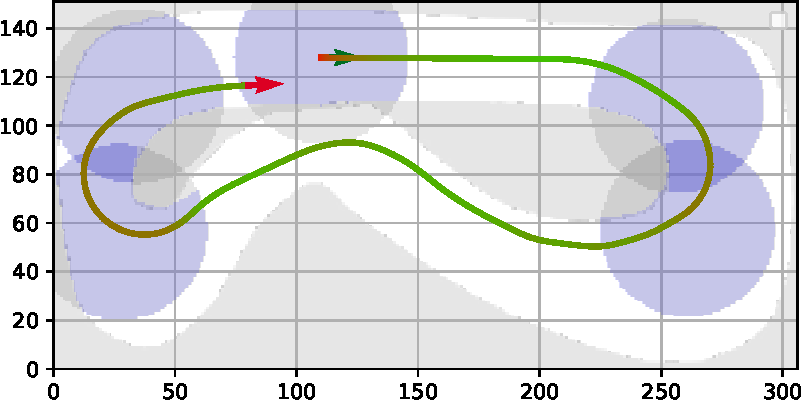
\includegraphics[width=\textwidth]{../img/experiments/porto_hybrid_astar_trajectory}
		\end{subfigure}
		\hfill
		\begin{subfigure}[c]{0.49\textwidth}
			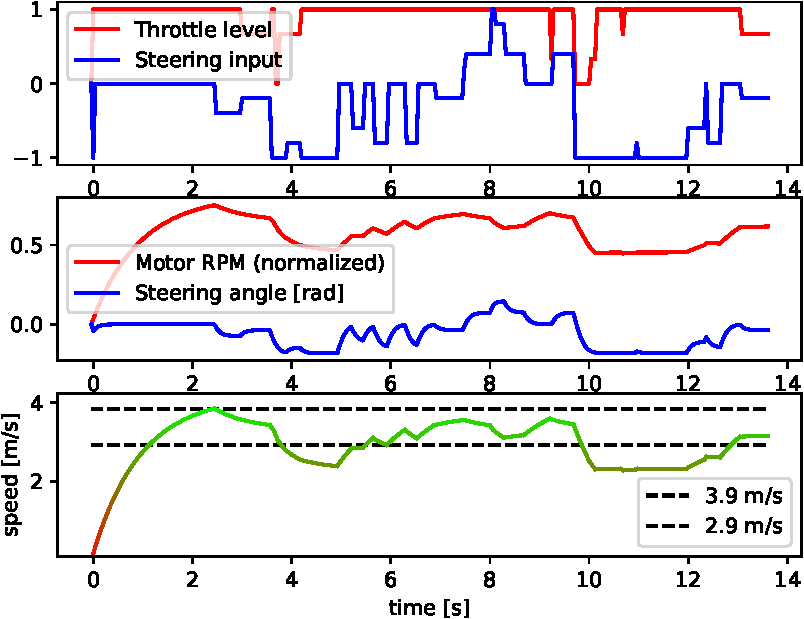
\includegraphics[width=\textwidth]{../img/experiments/porto_hybrid_astar_actuators}
		\end{subfigure}
		\caption{Solution found by Hybrid A* in \SI{192.30}{\milli\second}}
		\label{fig:solution_porto-hybrid_astar}	
	\end{subfigure}
	
	\vspace{0.5cm}
	
	\begin{subfigure}[t]{\textwidth}
		\begin{subfigure}[c]{0.49\textwidth}
			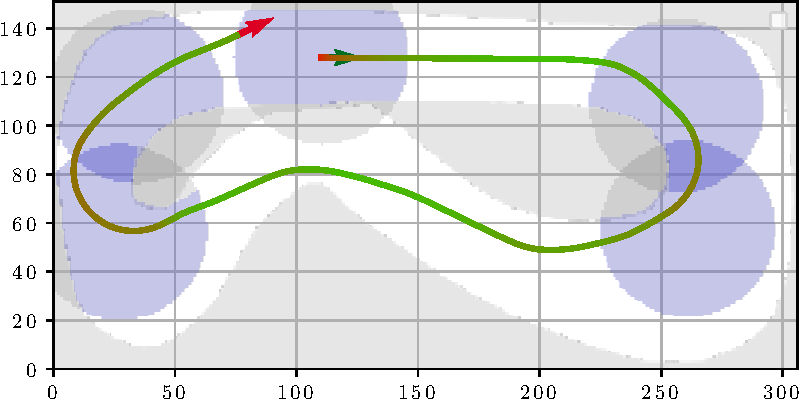
\includegraphics[width=\textwidth]{../img/experiments/porto_sehs_trajectory}
		\end{subfigure}
		\hfill
		\begin{subfigure}[c]{0.49\textwidth}
			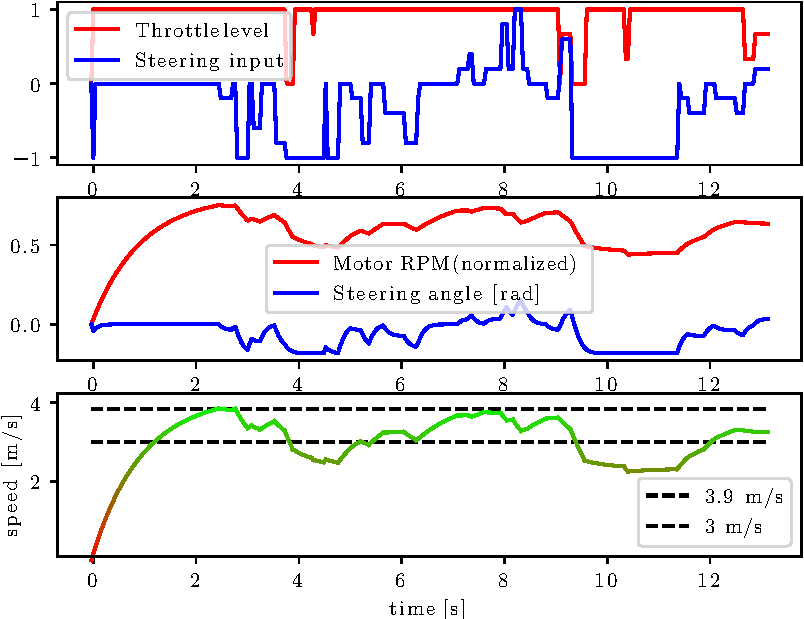
\includegraphics[width=\textwidth]{../img/experiments/porto_sehs_actuators}
		\end{subfigure}
		\caption{Solution found by SEHS in \SI{253.60}{\milli\second}}
		\label{fig:solution_porto-sehs}
	\end{subfigure}
	
	\vspace{0.75cm}
	
	\begin{subfigure}[t]{\textwidth}
		\centering
		\robustify\bfseries
		\begin{tabular}{c c c c S[detect-weight,table-format=7.0] S[detect-weight] S[detect-weight,table-format=2.2]}%
			\toprule
			Available & \multicolumn{3}{c}{Discretization} & \multicolumn{1}{c}{Opened} & \multicolumn{1}{c}{Search time} & \multicolumn{1}{c}{Lap time} \\
			actions & $xy$ [\si{\meter}] & RPM & $\theta$ & \multicolumn{1}{c}{nodes} & \multicolumn{1}{c}{[\si{\milli\second}]} & \multicolumn{1}{c}{[\si{\second}]} \\
			\midrule
			44 & 1.80 & 20 & 18 & \bfseries 67301 & \bfseries 192.30 & 13.64 \\
			248 & 1.44 & 20 & 36 & 838926 & 2544.00 & \bfseries 12.28 \\
			\bottomrule
		\end{tabular}
		\caption{Hybrid A* found both a trajectory in the least amount of time and also a trajectory with the best lap time.}
		\label{table:porto-hybrid_astar}
	\end{subfigure}
	
	\vspace{0.5cm}

	\begin{subfigure}[t]{\textwidth}
		\centering
		\robustify\bfseries
		\begin{tabular}{c c c c S[detect-weight,table-format=7.0] S[detect-weight] S[detect-weight,table-format=2.2]}%
			\toprule
			Available & \multicolumn{3}{c}{Discretization} & \multicolumn{1}{c}{Opened} & \multicolumn{1}{c}{Search time} & \multicolumn{1}{c}{Lap time} \\
			actions & Circles & RPM & $\theta$ & \multicolumn{1}{c}{nodes} & \multicolumn{1}{c}{[\si{\milli\second}]} & \multicolumn{1}{c}{[\si{\second}]} \\
			\midrule
			44 & 71 & 20 & 18 & 80763 & 253.60 & 13.16 \\
			84 & 71 & 80 & 36 & 1054427 & 2171.60 & 12.48 \\
			\bottomrule
		\end{tabular}
		\caption{SEHS could not find a solution faster nor could it find a better solution than Hybrid A* with any of the tested combination of parameters.}
		\label{table:porto-sehs}
	\end{subfigure}
	
	\vspace{0.75cm}
	
	\caption{Circuit ``Porto'' is a simple track which was inspired by the track used in the 2018 F1/10 competition in Porto.}
	\label{fig:porto}
\end{figure}

\begin{figure}[!tbp]%
	\centering
	
	\begin{subfigure}[t]{\textwidth}
		\begin{subfigure}[c]{0.49\textwidth}
			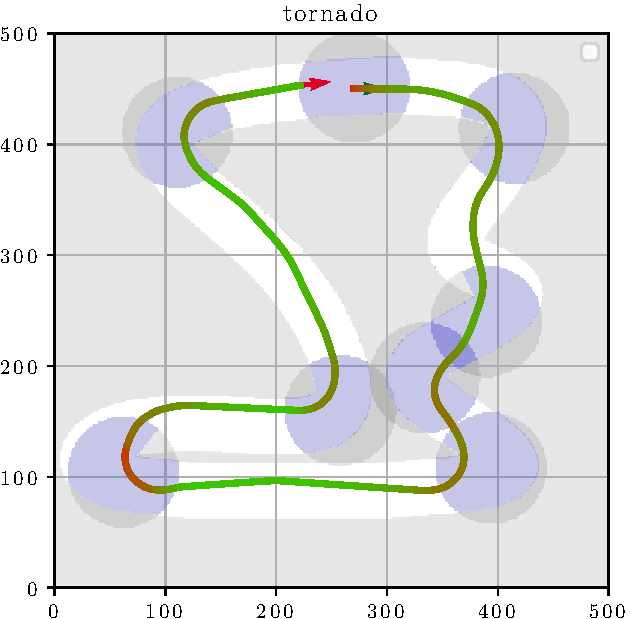
\includegraphics[width=\textwidth]{../img/experiments/tornado_hybrid_astar_trajectory}
		\end{subfigure}
		\hfill
		\begin{subfigure}[c]{0.49\textwidth}
			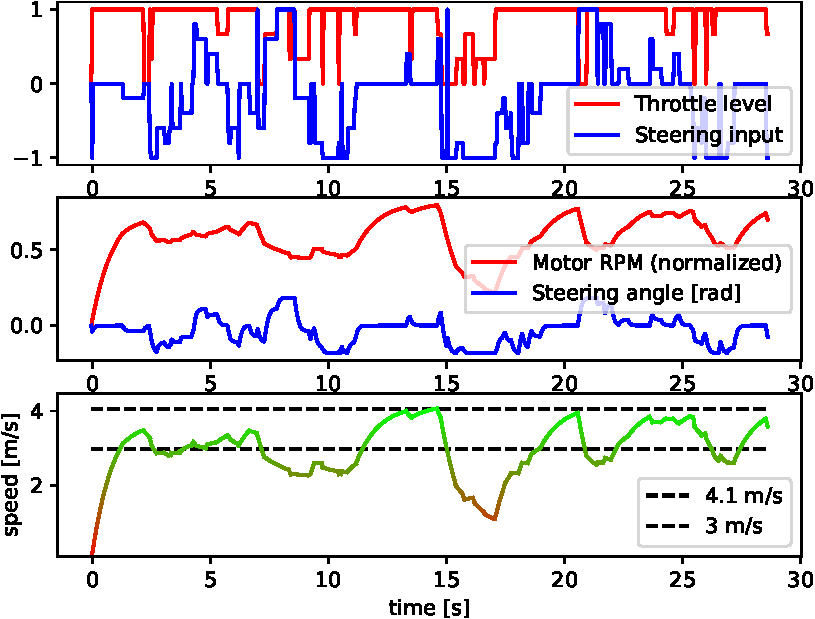
\includegraphics[width=\textwidth]{../img/experiments/tornado_hybrid_astar_actuators}
		\end{subfigure}
		\caption{Solution found by Hybrid A* in \SI{494.50}{\milli\second}}
		\label{fig:solution_tornado-hybrid_astar}	
	\end{subfigure}
	
	\vspace{0.75cm}
	
	\begin{subfigure}[t]{\textwidth}
		\begin{subfigure}[c]{0.49\textwidth}
			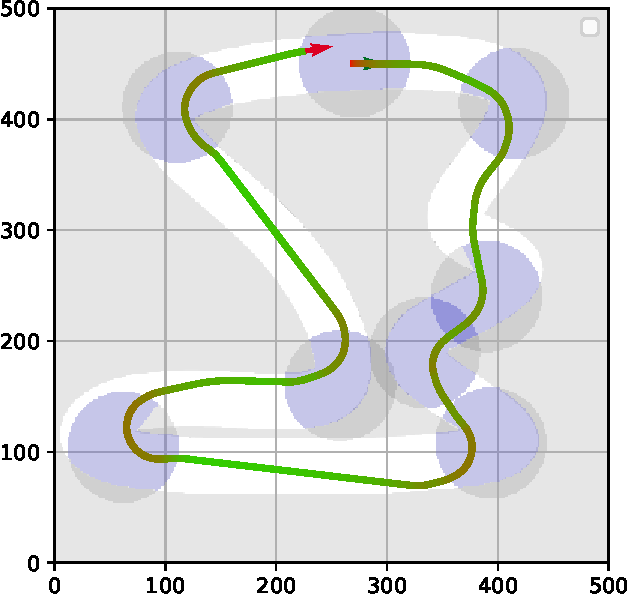
\includegraphics[width=\textwidth]{../img/experiments/tornado_sehs_trajectory}
		\end{subfigure}
		\hfill
		\begin{subfigure}[c]{0.49\textwidth}
			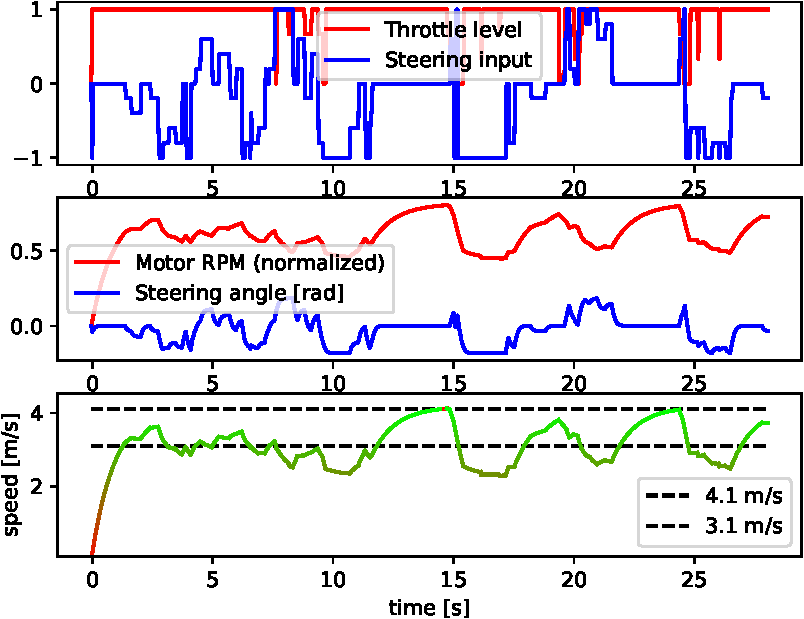
\includegraphics[width=\textwidth]{../img/experiments/tornado_sehs_actuators}
		\end{subfigure}
		\caption{Solution found by SEHS in \SI{551.30}{\milli\second}}
		\label{fig:solution_tornado-sehs}
	\end{subfigure}
	
	\vspace{0.75cm}
	
	\begin{subfigure}[t]{\textwidth}
		\centering
		\robustify\bfseries
		\begin{tabular}{c c c c S[detect-weight,table-format=7.0] S[detect-weight] S[detect-weight,table-format=2.2]}%
			\toprule
			Available & \multicolumn{3}{c}{Discretization} & \multicolumn{1}{c}{Opened} & \multicolumn{1}{c}{Search time} & \multicolumn{1}{c}{Lap time} \\
			actions & $xy$ [\si{\meter}] & RPM & $\theta$ & \multicolumn{1}{c}{nodes} & \multicolumn{1}{c}{[\si{\milli\second}]} & \multicolumn{1}{c}{[\si{\second}]} \\
			\midrule
			44 & 1.44 & 20 & 18 & 177778 & \bfseries 494.50 & 28.64 \\
			84 & 1.44 & 80 & 52 & 3464766 & 6611.70 & \bfseries 26.24 \\
			\bottomrule
		\end{tabular}
		\caption{Hybrid A* results}
		\label{table:tornado-hybrid_astar}
	\end{subfigure}
	
	\vspace{0.5cm}
	
	\begin{subfigure}[t]{\textwidth}
		\centering
		\robustify\bfseries
		\begin{tabular}{c c c c S[detect-weight,table-format=7.0] S[detect-weight] S[detect-weight,table-format=2.2]}%
			\toprule
			Available & \multicolumn{3}{c}{Discretization} & \multicolumn{1}{c}{Opened} & \multicolumn{1}{c}{Search time} & \multicolumn{1}{c}{Lap time} \\
			actions & Circles & RPM & $\theta$ & \multicolumn{1}{c}{nodes} & \multicolumn{1}{c}{[\si{\milli\second}]} & \multicolumn{1}{c}{[\si{\second}]} \\
			\midrule
			44 & 126 & 20 & 18 & \bfseries 144864 & 551.30 & 28.08 \\
			84 & 126 & 80 & 52 & 2827948 & 6397.60 & 26.84 \\
			\bottomrule
		\end{tabular}
		\caption{SEHS results}
		\label{table:tornado-sehs}
	\end{subfigure}
	
	\vspace{0.75cm}
	
	\caption{Circuit ``Tornado''}
	\label{fig:tornado}
\end{figure}

\begin{figure}[!tbp]%
	\centering
	
	\begin{subfigure}[t]{\textwidth}
		\begin{subfigure}[c]{0.49\textwidth}
			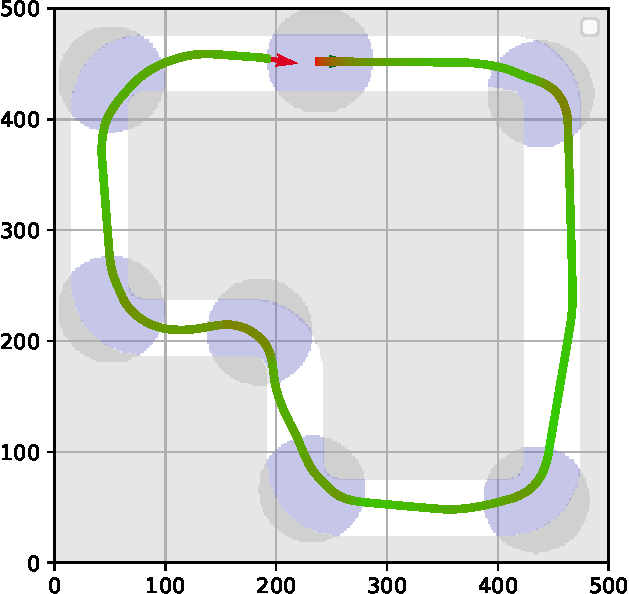
\includegraphics[width=\textwidth]{../img/experiments/simple_hybrid_astar_trajectory}
		\end{subfigure}
		\hfill
		\begin{subfigure}[c]{0.49\textwidth}
			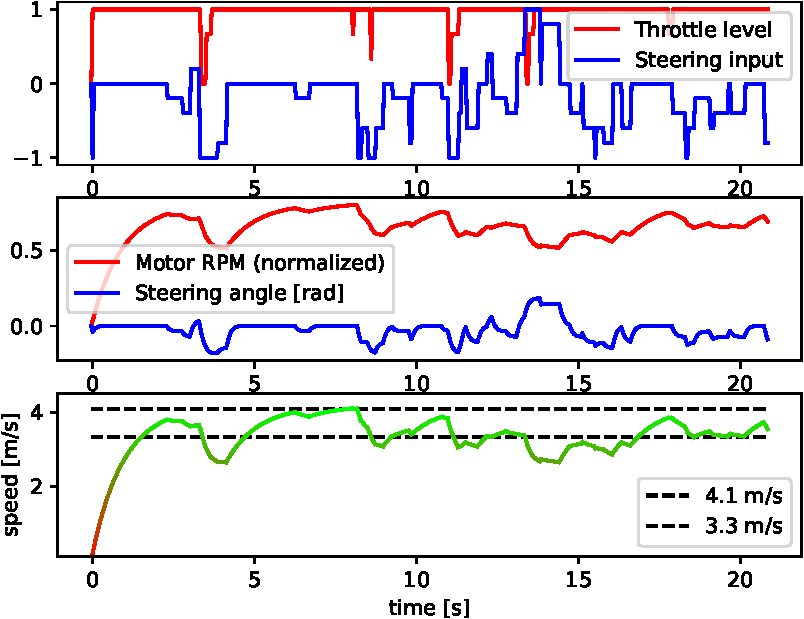
\includegraphics[width=\textwidth]{../img/experiments/simple_hybrid_astar_actuators}
		\end{subfigure}
		\caption{Solution found by Hybrid A* in \SI{236.20}{\milli\second}}
		\label{fig:simple-hybrid_astar}
	\end{subfigure}
	
	\vspace{0.75cm}
	
	\begin{subfigure}[t]{\textwidth}
		\begin{subfigure}[c]{0.49\textwidth}
			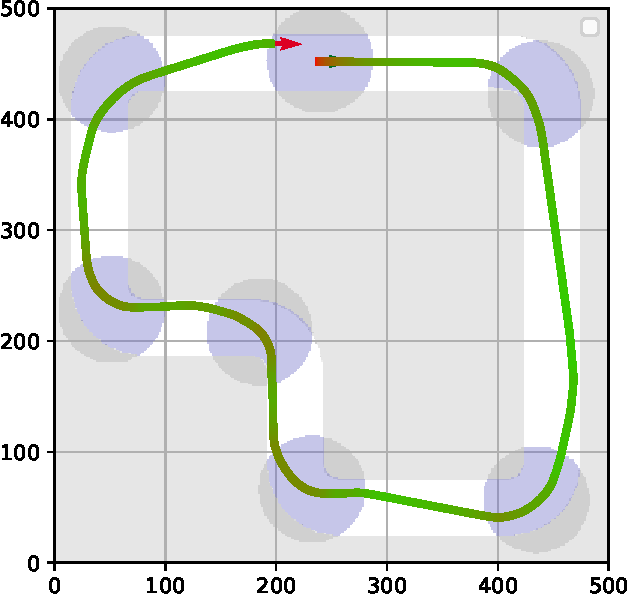
\includegraphics[width=\textwidth]{../img/experiments/simple_sehs_trajectory}
		\end{subfigure}
		\hfill
		\begin{subfigure}[c]{0.49\textwidth}
			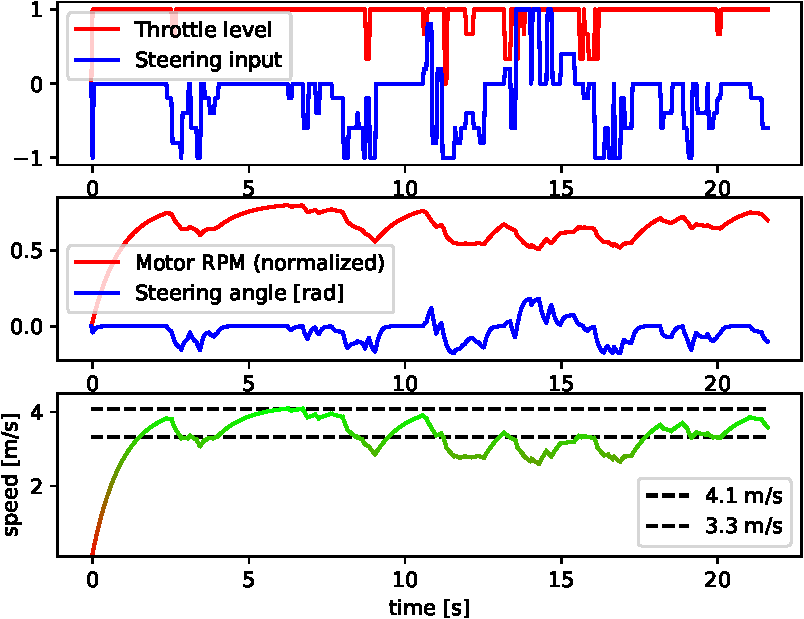
\includegraphics[width=\textwidth]{../img/experiments/simple_sehs_actuators}
		\end{subfigure}
		\caption{Soultion found by SEHS in \SI{449.20}{\milli\second}}
		\label{fig:simple-sehs}
	\end{subfigure}
	
	\vspace{0.75cm}
	
	\begin{subfigure}[t]{\textwidth}
		\centering
		\robustify\bfseries
		\begin{tabular}{c c c c S[detect-weight,table-format=7.0] S[detect-weight] S[detect-weight,table-format=2.2]}%
			\toprule
			Available & \multicolumn{3}{c}{Discretization} & \multicolumn{1}{c}{Opened} & \multicolumn{1}{c}{Search time} & \multicolumn{1}{c}{Lap time} \\
			actions & $xy$ [\si{\meter}] & RPM & $\theta$ & \multicolumn{1}{c}{nodes} & \multicolumn{1}{c}{[\si{\milli\second}]} & \multicolumn{1}{c}{[\si{\second}]} \\
			\midrule
			44 & 1.80 & 20 & 18 & \bfseries 78401 & \bfseries 236.20 & 20.88 \\
			84 & 1.44 & 40 & 36 & 807771 & 1926.50 & 19.92 \\
			\bottomrule
		\end{tabular}
		\caption{Hybrid A* results}
		\label{table:simple-hybrid_astar}
	\end{subfigure}
	
	\vspace{0.5cm}

	\begin{subfigure}[t]{\textwidth}
		\centering
		\robustify\bfseries
		\begin{tabular}{c c c c S[detect-weight,table-format=7.0] S[detect-weight] S[detect-weight,table-format=2.2]}%
			\toprule
			Available & \multicolumn{3}{c}{Discretization} & \multicolumn{1}{c}{Opened} & \multicolumn{1}{c}{Search time} & \multicolumn{1}{c}{Lap time} \\
			actions & Circles & RPM & $\theta$ & \multicolumn{1}{c}{nodes} & \multicolumn{1}{c}{[\si{\milli\second}]} & \multicolumn{1}{c}{[\si{\second}]} \\
			\midrule
			44 & 134 & 20 & 18 & 129796 & 449.20 & 21.64 \\
			88 & 134 & 40 & 52 & 1443863 & 4204.30 & \bfseries 19.76 \\
			\bottomrule
		\end{tabular}
		\caption{SEHS results}
		\label{table:simple-sehs}
	\end{subfigure}
	
	\vspace{0.75cm}
	
	\caption{Circuit ``Simple''}
	\label{fig:simple}
\end{figure}

\begin{figure}[!tbp]%
	\centering
	
	\begin{subfigure}[t]{\textwidth}
		\begin{subfigure}[c]{0.49\textwidth}
			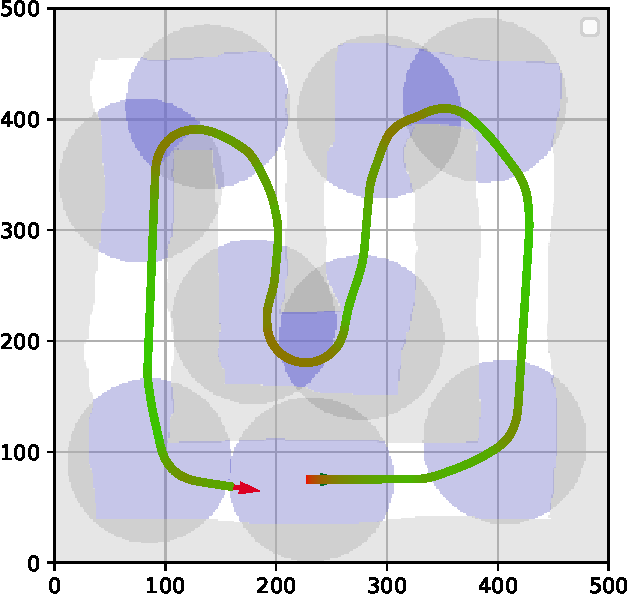
\includegraphics[width=\textwidth]{../img/experiments/u_hybrid_astar_trajectory}
		\end{subfigure}
		\hfill
		\begin{subfigure}[c]{0.49\textwidth}
			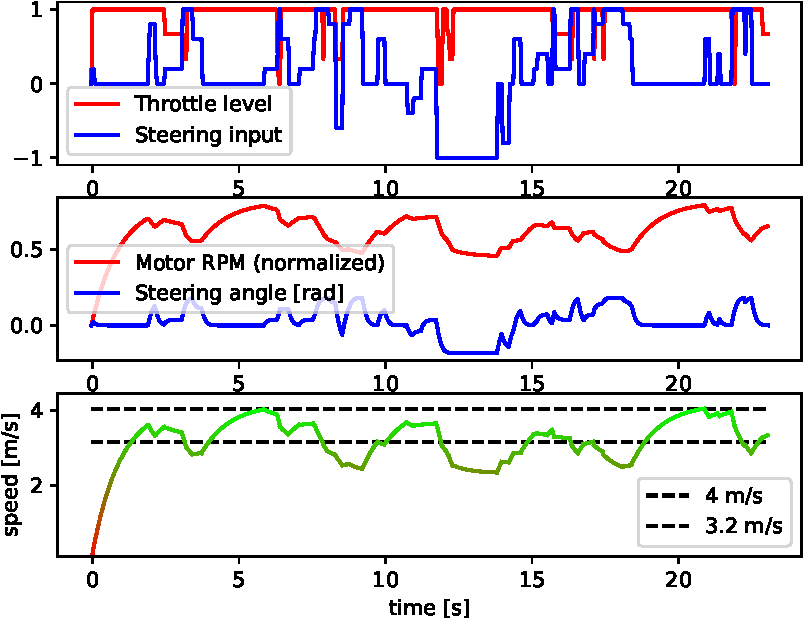
\includegraphics[width=\textwidth]{../img/experiments/u_hybrid_astar_actuators}
		\end{subfigure}	
		\caption{Solution found by Hybrid A* in \SI{440.10}{\milli\second}}
		\label{fig:u-hybrid_astar}
	\end{subfigure}
	
	\vspace{0.75cm}
	
	\begin{subfigure}[t]{\textwidth}
		\begin{subfigure}[c]{0.49\textwidth}
			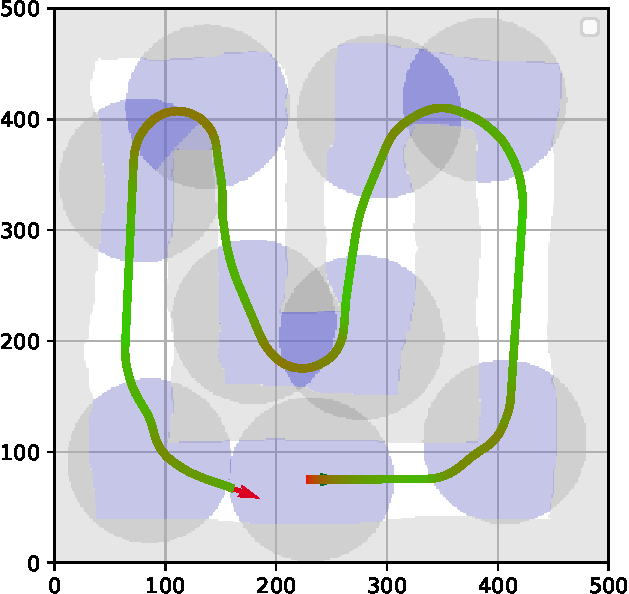
\includegraphics[width=\textwidth]{../img/experiments/u_sehs_trajectory}
		\end{subfigure}
		\hfill
		\begin{subfigure}[c]{0.49\textwidth}
			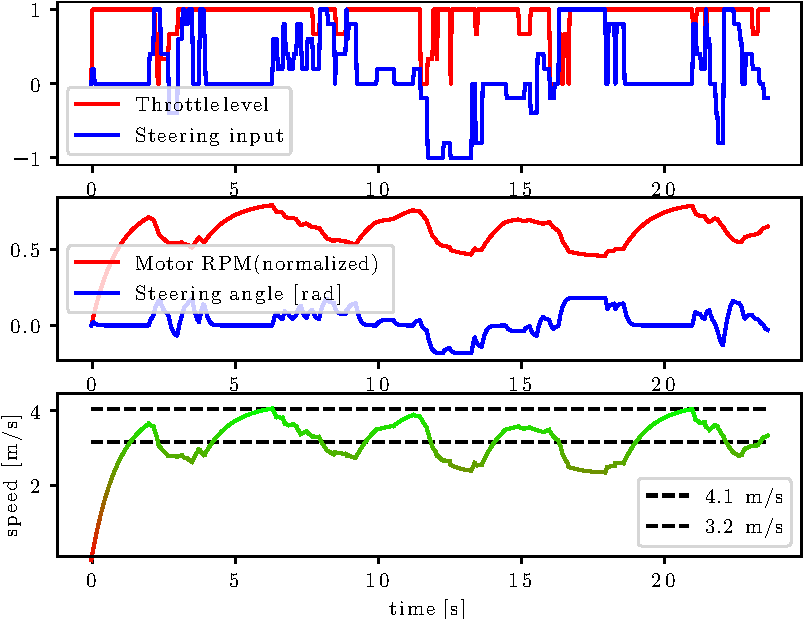
\includegraphics[width=\textwidth]{../img/experiments/u_sehs_actuators}
		\end{subfigure}
		\caption{Solution found by SEHS in \SI{533.60}{\milli\second}}
		\label{fig:u-sehs}
	\end{subfigure}
	
	\vspace{0.75cm}
	
	\begin{subfigure}[t]{\textwidth}
		\centering
		\robustify\bfseries
		\begin{tabular}{c c c c S[detect-weight,table-format=7.0] S[detect-weight] S[detect-weight,table-format=2.2]}%
			\toprule
			Available & \multicolumn{3}{c}{Discretization} & \multicolumn{1}{c}{Opened} & \multicolumn{1}{c}{Search time} & \multicolumn{1}{c}{Lap time} \\
			actions & $xy$ [\si{\meter}] & RPM & $\theta$ & \multicolumn{1}{c}{nodes} & \multicolumn{1}{c}{[\si{\milli\second}]} & \multicolumn{1}{c}{[\si{\second}]} \\
			\midrule
			44 & 1.80 & 20 & 18 & \bfseries 145240 & \bfseries 440.10 & 23.08 \\
			84 & 1.44 & 40 & 36 & 1442255 & 3667.90 & 21.84 \\
			\bottomrule
		\end{tabular}
		\caption{Hybrid A* results}
		\label{table:u-hybrid_astar}
	\end{subfigure}
	
	\vspace{0.5cm}

	\begin{subfigure}[t]{\textwidth}
		\centering
		\robustify\bfseries
		\begin{tabular}{c c c c S[detect-weight,table-format=7.0] S[detect-weight] S[detect-weight,table-format=2.2]}%
			\toprule
			Available & \multicolumn{3}{c}{Discretization} & \multicolumn{1}{c}{Opened} & \multicolumn{1}{c}{Search time} & \multicolumn{1}{c}{Lap time} \\
			actions & Circles & RPM & $\theta$ & \multicolumn{1}{c}{nodes} & \multicolumn{1}{c}{[\si{\milli\second}]} & \multicolumn{1}{c}{[\si{\second}]} \\
			\midrule
			44 & 123 & 20 & 18 & 147605 & 533.60 & 23.64 \\
			44 & 123 & 40 & 52 & 829326 & 2289.80 & \bfseries 21.60 \\
			\bottomrule
		\end{tabular}
		\caption{SEHS results}
		\label{table:u-sehs}
	\end{subfigure}
	
	\vspace{0.75cm}
	
	\caption{Circuit ``U''}
	\label{fig:u}
\end{figure}

\begin{figure}[!tbp]%
	\centering
	
	\begin{subfigure}[t]{\textwidth}
		\begin{subfigure}[c]{0.49\textwidth}
			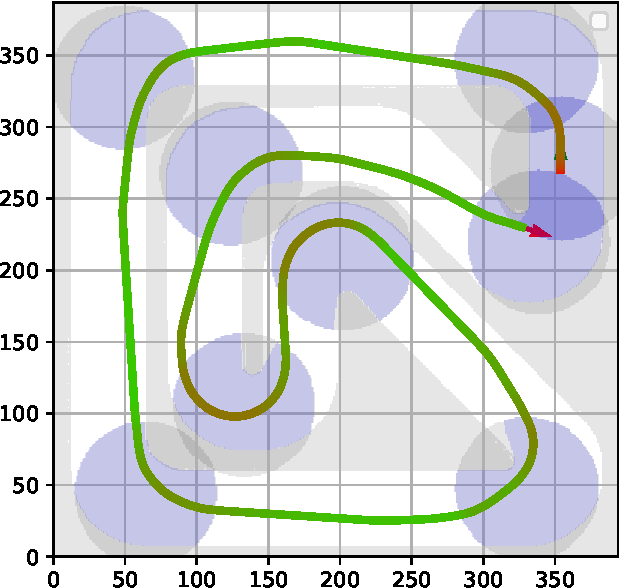
\includegraphics[width=\textwidth]{../img/experiments/race_track_hybrid_astar_trajectory}
		\end{subfigure}
		\hfill
		\begin{subfigure}[c]{0.49\textwidth}
			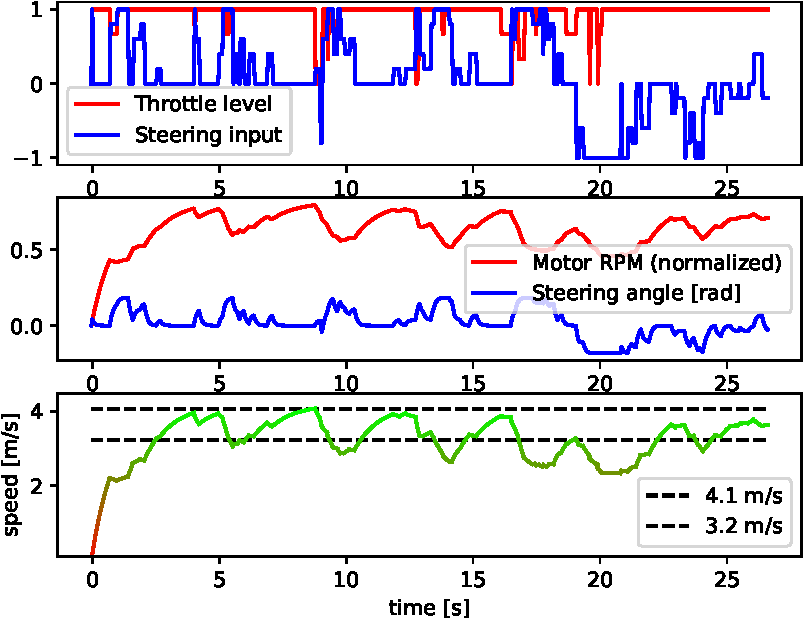
\includegraphics[width=\textwidth]{../img/experiments/race_track_hybrid_astar_actuators}
		\end{subfigure}	
		\caption{Solution found by Hybrid A* in \SI{570.30}{\milli\second}}
		\label{fig:race_track-hybrid_astar}
	\end{subfigure}
	
	\vspace{0.75cm}
	
	\begin{subfigure}[t]{\textwidth}
		\begin{subfigure}[c]{0.49\textwidth}
			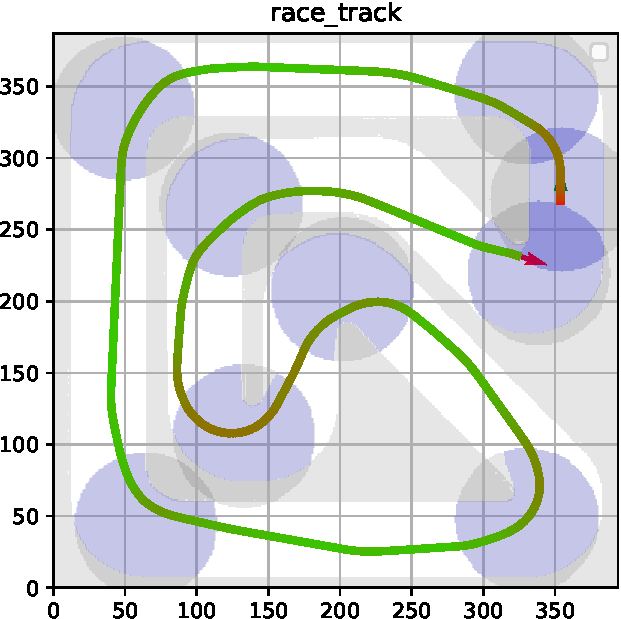
\includegraphics[width=\textwidth]{../img/experiments/race_track_sehs_trajectory}
		\end{subfigure}
		\hfill
		\begin{subfigure}[c]{0.49\textwidth}
			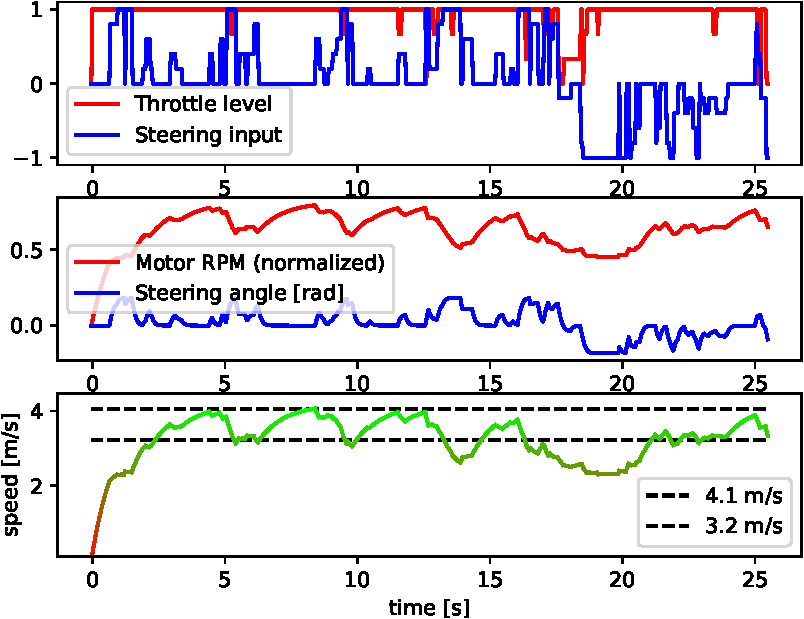
\includegraphics[width=\textwidth]{../img/experiments/race_track_sehs_actuators}
		\end{subfigure}
		\caption{Solution found by SEHS in \SI{598.10}{\milli\second}}
		\label{fig:race_track-sehs}
	\end{subfigure}
	
	\vspace{0.75cm}
	
	\begin{subfigure}[t]{\textwidth}
		\centering
		\robustify\bfseries
		\begin{tabular}{c c c c S[detect-weight,table-format=7.0] S[detect-weight] S[detect-weight,table-format=2.2]}%
			\toprule
			Available & \multicolumn{3}{c}{Discretization} & \multicolumn{1}{c}{Opened} & \multicolumn{1}{c}{Search time} & \multicolumn{1}{c}{Lap time} \\
			actions & $xy$ [\si{\meter}] & RPM & $\theta$ & \multicolumn{1}{c}{nodes} & \multicolumn{1}{c}{[\si{\milli\second}]} & \multicolumn{1}{c}{[\si{\second}]} \\
			\midrule
			44 & 1.80 & 20 & 36 & 195755 & \bfseries 570.30 & 26.64 \\
			84 & 1.80 & 80 & 36 & 1450767 & 2749.70 & 25.48 \\
			\bottomrule
		\end{tabular}
		\caption{Hybrid A* performed worse when compared to SEHS for this track.}
		\label{table:race_track-hybrid_astar}
	\end{subfigure}
	
	\vspace{0.5cm}

	\begin{subfigure}[t]{\textwidth}
		\centering
		\robustify\bfseries
		\begin{tabular}{c c c c S[detect-weight,table-format=7.0] S[detect-weight] S[detect-weight,table-format=2.2]}%
			\toprule
			Available & \multicolumn{3}{c}{Discretization} & \multicolumn{1}{c}{Opened} & \multicolumn{1}{c}{Search time} & \multicolumn{1}{c}{Lap time} \\
			actions & Circles & RPM & $\theta$ & \multicolumn{1}{c}{nodes} & \multicolumn{1}{c}{[\si{\milli\second}]} & \multicolumn{1}{c}{[\si{\second}]} \\
			\midrule
			44 & 164 & 20 & 18 & \bfseries 169002 & 598.10 & 25.52 \\
			124 & 164 & 20 & 52 & 1277382 & 4809.20 & \bfseries 25.04 \\
			\bottomrule
		\end{tabular}
		\caption{The solution found by the fastest lap time. Of the two solutions with the lowest computation time, the solution found by SEHS has a significantly better lap time.}
		\label{table:race_track-sehs}
	\end{subfigure}
	
	\vspace{0.25cm}
	
	\caption{Circuit ``Race Track''}
	\label{fig:race_track}
\end{figure}

\begin{figure}[!tbp]%
	\centering
	
	\begin{subfigure}[t]{\textwidth}
		\begin{subfigure}[c]{0.49\textwidth}
			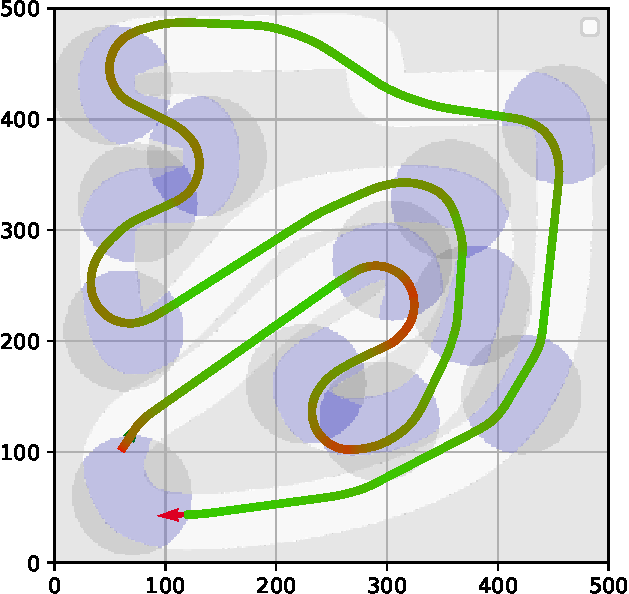
\includegraphics[width=\textwidth]{../img/experiments/zurich_hybrid_astar_trajectory.pdf}
		\end{subfigure}
		\hfill
		\begin{subfigure}[c]{0.49\textwidth}
			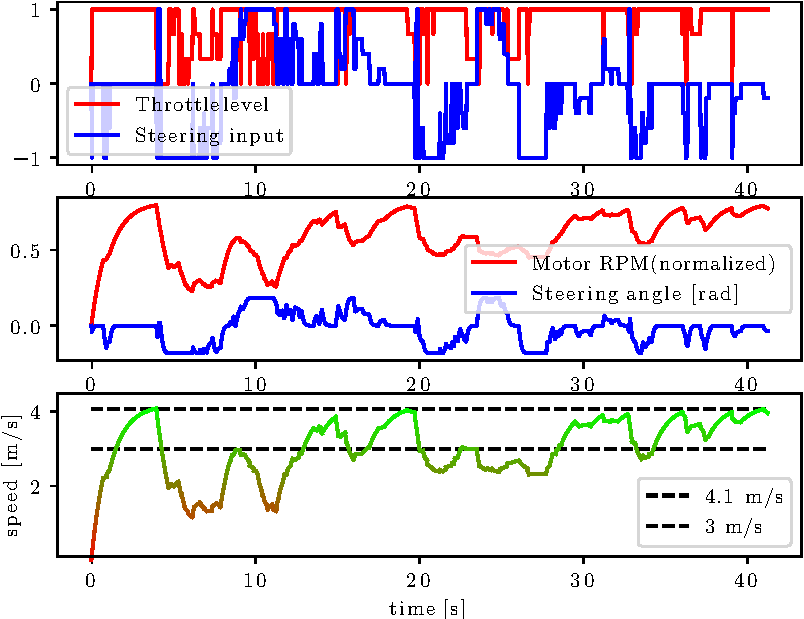
\includegraphics[width=\textwidth]{../img/experiments/zurich_hybrid_astar_actuators}
		\end{subfigure}
		\caption{Solution found by Hybrid A* in \SI{1041.10}{\milli\second}}
		\label{fig:zurich-hybrid_astar}
	\end{subfigure}
	
	\vspace{0.75cm}
	
	\begin{subfigure}[t]{\textwidth}
		\centering
		\robustify\bfseries
		\begin{tabular}{c c c c S[detect-weight,table-format=7.0] S[detect-weight] S[detect-weight,table-format=2.2]}%
			\toprule
			Available & \multicolumn{3}{c}{Discretization} & \multicolumn{1}{c}{Opened} & \multicolumn{1}{c}{Search time} & \multicolumn{1}{c}{Lap time} \\
			actions & $xy$ [\si{\meter}] & RPM & $\theta$ & \multicolumn{1}{c}{nodes} & \multicolumn{1}{c}{[\si{\milli\second}]} & \multicolumn{1}{c}{[\si{\second}]} \\
			\midrule
			44 & 1.80 & 40 & 36 & 488873 & 1041.10 & 41.28 \\
			88 & 1.80 & 80 & 36 & 1922591 & 3811.00 & 38.52 \\
			\bottomrule
		\end{tabular}
		\caption{Hybrid A* was the only algorithm of the two which found a solution. The SEHS algorithm did not find any solution for any combination of the parameters.}
		\label{table:zurich-hybrid_astar}
	\end{subfigure}
	
	\vspace{0.75cm}
	
	\caption{Circuit ``Zurich''}
	\label{fig:zurich}
\end{figure}

\section{Autonomous Race}

To further test the algorithms, we implemented the complete Artificial Racing Agent on top of the \gls{ROS} and we built a custom hardware inspired by the F1/10 platform. The details of the implementation are described in the appendixes Experimental Vehicle (Appendix~\ref{chapter:hardware}) and Technical Documentation (Appendix~\ref{chapter:technical_documentation}).

In the following experiments, we tried to test the racing capabilities of the vehicle. The vehicle was given a complete map of the circuit at the beginning of the race. The goal was to go around the circuit repeatedly without colliding with walls and obstacles and reaching the best lap times as possible.

The agent repeatedly triggers the \gls{SEHS} based trajectory planning algorithm from the latest known state of the vehicle with the latest known state of the map with the obstacles marked in it through the current list of waypoints. At the same time, the vehicle is already driving and following the last published trajectory. Once the planning algorithm comes up with a new plan, it replaces the old plan and it can start planning again with the latest known state.

\subsection{Testing Criteria}
For the planning algorithm to be viable, it must calculate the trajectory in a short period of time before the vehicle physically moves to the end of the previous trajectory. We were also interested in the safety of the planned trajectory and the distance the vehicle keeps from the obstacles while following the trajectory. Finally, our goal is to achieve fast lap times and we are interested in the maximum speed our vehicle can achieve while driving safely.

\subsection{Real World Testing}

\begin{figure}
	\centering
	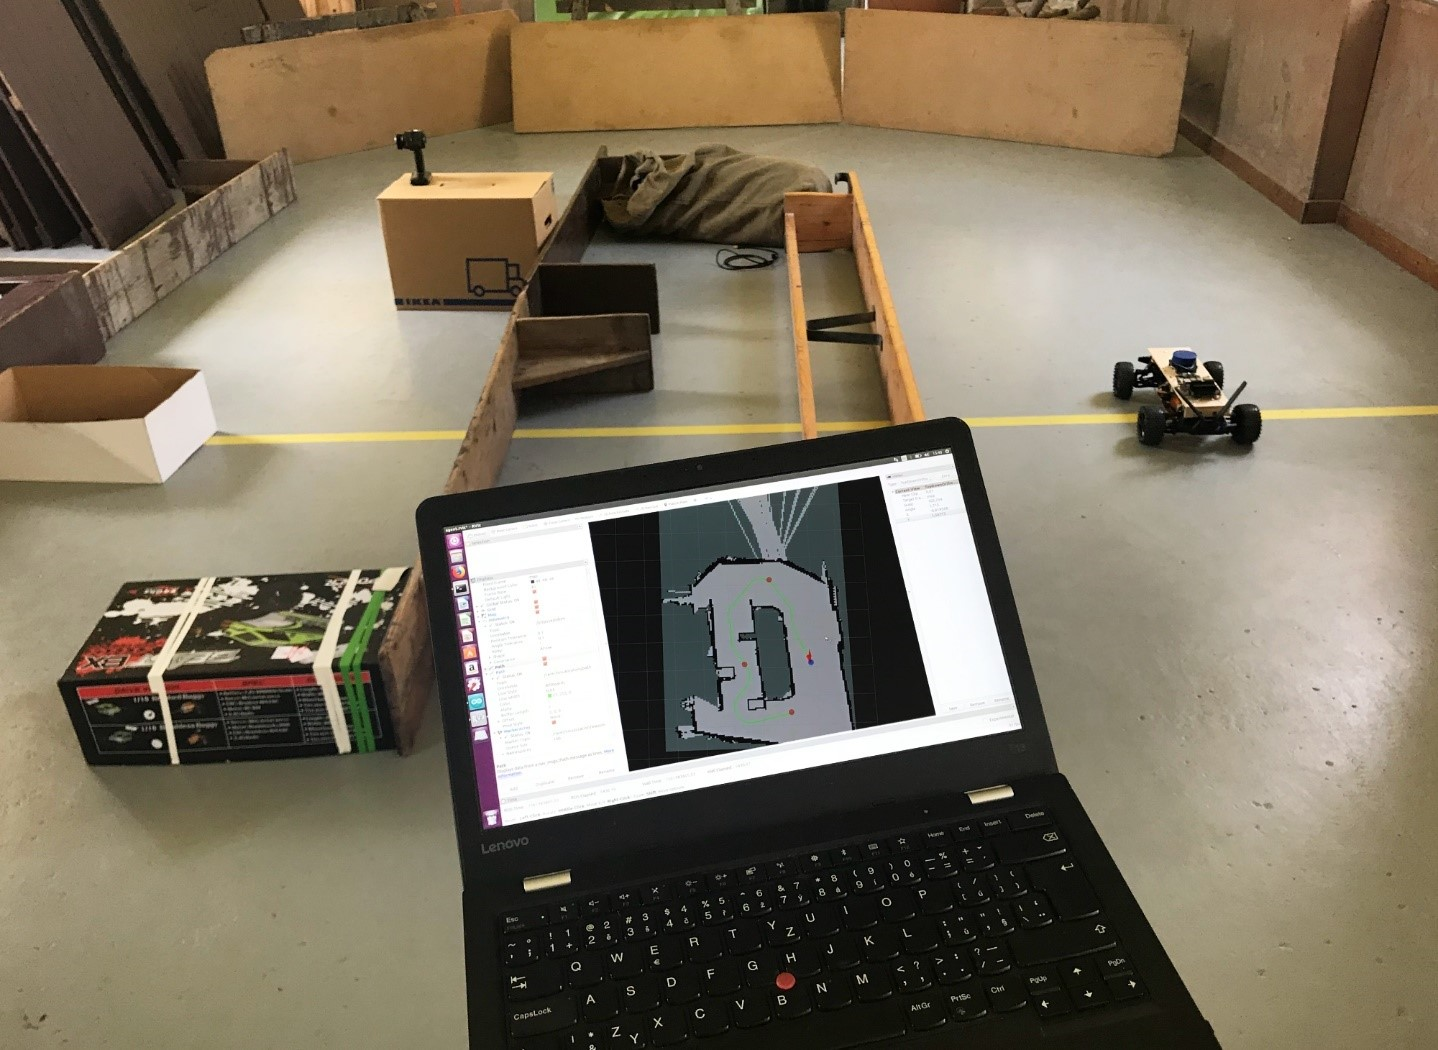
\includegraphics[width=\textwidth]{../img/experiments/real-world-still.jpg}
	\caption{The planning algorithm finds a trajectory from the last known state of the vehicle through the waypoints ahead of it while avoiding the obstacles marked in the map.}
	\label{fig:real-world-testing-still}
\end{figure}


Initially we wanted to perform tests outdoors on an asphalt road, but it proved problematic because of surface curvature and slope and because of unstable weather conditions. Another unexpected problem we had to solve was a problem with the \gls*{LIDAR} unit. It performed very unreliably in direct sunlight. In the end, we tested our vehicle indoors in a rectangular gym \SI{10}{\meter} long and \SI{6}{\meter} wide with concrete surface which was available to us for several days. We built several versions of an obstacle course using gym equipment and from cardboard boxes. One such circuit is shown in Figure~\ref{fig:real-world-testing-still}.

The experiment consisted of two phases. First, we built a 2D map from the data coming from the \gls*{LIDAR} as the vehicle drove around the track using a remote controller. Using this map, we assembled a configuration file describing the racing circuit. Next, we started all the \gls{ROS} nodes for vehicle state monitoring, circuit progress monitoring, trajectory planning, and trajectory following. Once the planning algorithm produced the first trajectory, the vehicle started following it. We were closely monitoring the movement of the vehicle visually and using telemetry data on a laptop through the \texttt{Rviz} program\footnote{\url{http://wiki.ros.org/rviz}}. We were ready to take control of the vehicle using the remote control to prevent damage to the vehicle and to its surroundings at all times. Any input from the controller would cancel the autonomous mode and switch the vehicle into a remote-control mode. The vehicle then stayed in this mode until a button on the vehicle was physically pressed.

We struggled with unreliable odometry data for several days. We tested several different localization libraries, adjusted data we collected from the sensors, and tweaked the parameters of the libraries until we were able to get usable odometry data at least at low speeds. At higher speeds, the vehicle would quickly lose track of its actual position and orientation on the map and it would collide with a wall or with an obstacle.

By the end of the testing, the vehicle was able to reliably circle around the track without hitting obstacles and without the odometry significantly diverging from the actual state of the vehicle. The car repeatedly completed a circuit which was approximately 20 meters long in 15 seconds at the steady speed of \SI{1.3}{\meter\per\second}~(\SI{4.68}{\kilo\meter\per\hour}) which corresponds to the speed of \SI{46.8}{\kilo\meter\per\hour} of a full-size vehicle. At this speed, the limitations of the kinematic model do not manifest, and the vehicle had no issues undershooting or overshooting turns. A photo from this test is shown in Figure~\ref{fig:real-world-testing-driving} and a video recording of this experiment is available in the attachment of this thesis \footnote{The videos are locaded in the \texttt{/experiments/experimental-vehicle-gym} folder in the thesis attachment.}.

\begin{figure}
	\centering
	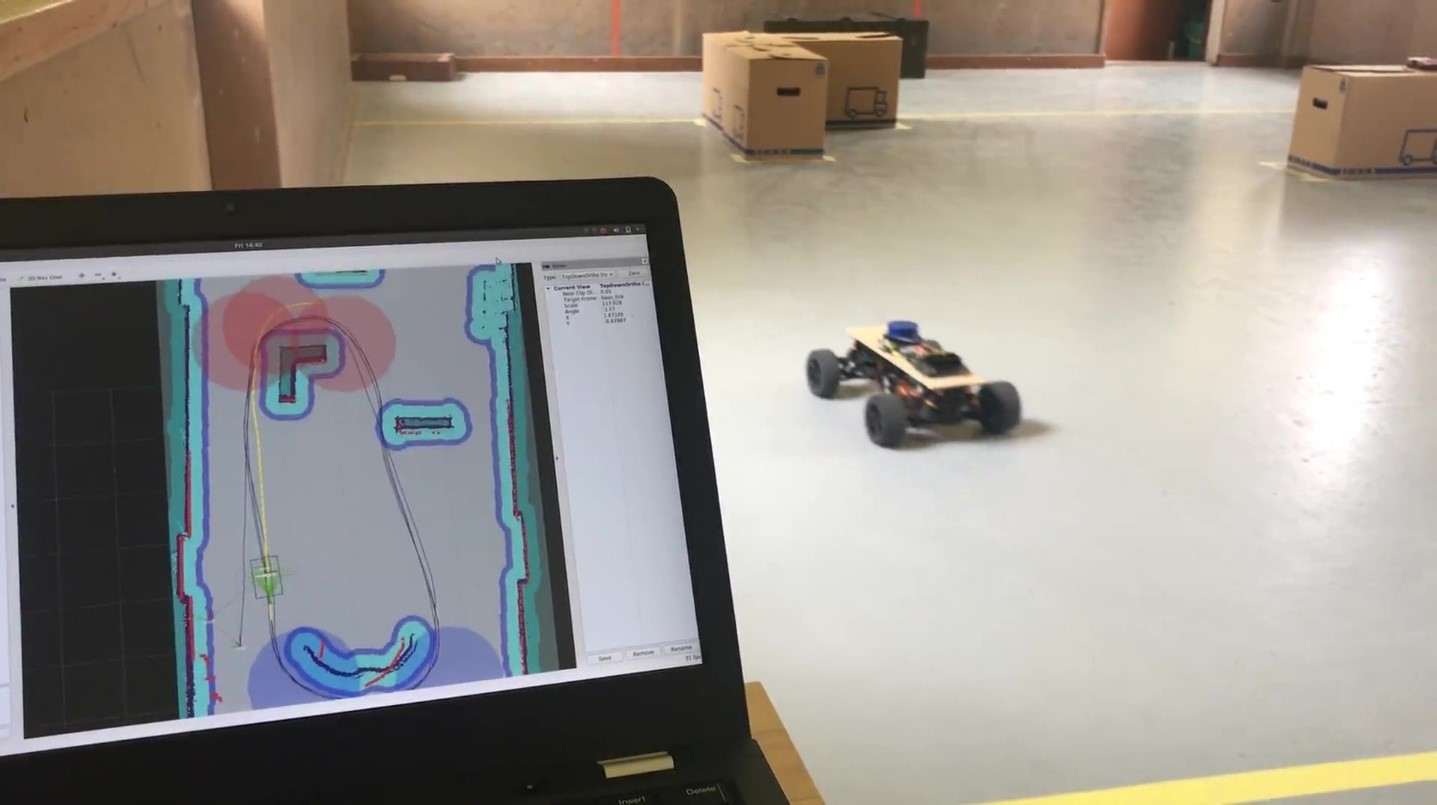
\includegraphics[width=\textwidth]{../img/experiments/real-world-driving.jpg}
	\caption{The vehicle is slowly driving along a circuit in a gym. The telemetry from the vehicle is monitored on a notebook connected to the vehicle over Wi-Fi.}
	\label{fig:real-world-testing-driving}
\end{figure}

The trajectory planning algorithm performed well even with just the low-powered ARM processor and the vehicle had never reached the end of the planned trajectory before a new extended trajectory was published. The \gls{DWA} algorithm kept the vehicle on the track and avoided all cardboard boxes placed along the circuit.

Although the robot was able to navigate autonomously without any collisions, the speeds we were able to reach, without losing track of the position of the vehicle, were low and did not reach the speed at which we would start seeing any effects of high speed maneuvering, such as wheel slipping and skidding and overshooting corners. We were also unable to test evasion of dynamic obstacles because the obstacle detection library produced too many ghost obstacles from our noisy and low-frequency \gls*{LIDAR} scans.

\subsection{Simulator}
\label{sec:simulator}
Due to the hardware issues we ran into and due to other factors, which did not allow further improvements and testing of the vehicle during the spring of 2020, we conducted further experiments only with the Gazebo simulator \cite{gazebo} configured for the F1/10 platform \cite{varundev_ros_19}. This change gave us the opportunity to test the algorithm with perfect odometry, but with the same interface between the algorithm and the simulated actuators of the virtual vehicle. To adapt the algorithm for the simulator, we had to modify our steering servo and motor models. We tweaked the parameters of our models to predict the behavior of the simulated vehicle as closely as possible.

The F1/10 simulator repository contains a 3D map\footnote{To view the state of the repository at the time of writing, see \url{https://github.com/f1tenth-dev/simulator/tree/140f8bd93b22b59d7cf7bfa753e1fdc73a4a8e59}. The repository has changed since then and the map we used has been removed.} with several different types of corners and it is shown in Figure~\ref{fig:gazebo-track}. Especially the middle part which consists of a series of left-hand turn followed by a right-hand hairpin turn presents a challenge where the car must slow down to avoid collision while keeping as much speed as possible to still reach a good lap time. We ran the full-circuit planning for the modified vehicle model and for this track.

For this experiment, we turned off the obstacle detection and we focused only on the lap times in a track without any obstacles. We tried a reference implementation against our four different combinations of algorithms and for each of them, we let it run for up to 10 consecutive laps. We ran each algorithm three times and we used the run in which it was able to complete all of the 10 laps and in which it reached the best average lap time.

\begin{figure}
	\centering
	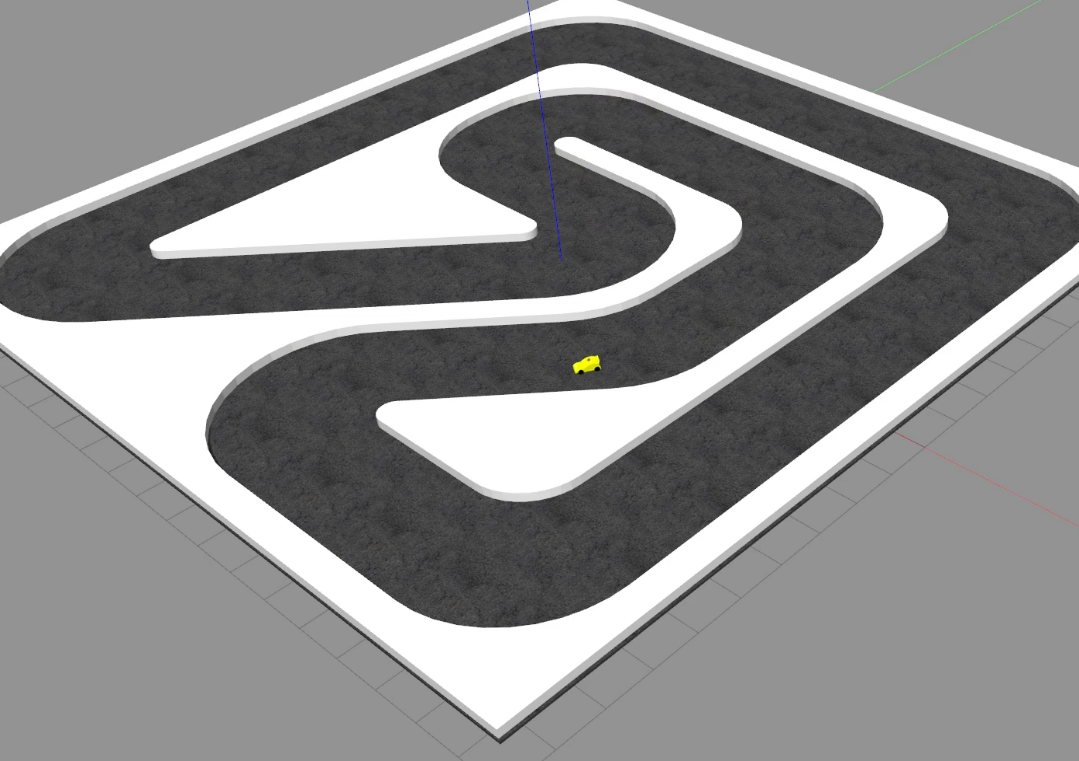
\includegraphics[width=0.75\textwidth]{../img/experiments/gazebo-track.png}
	\caption{The testing track contains several long straights and several challenging turns. The Gazebo simulator allows us to monitor and modify the 3D scene.}
	\label{fig:gazebo-track}
\end{figure}

\begin{figure}
	\centering
	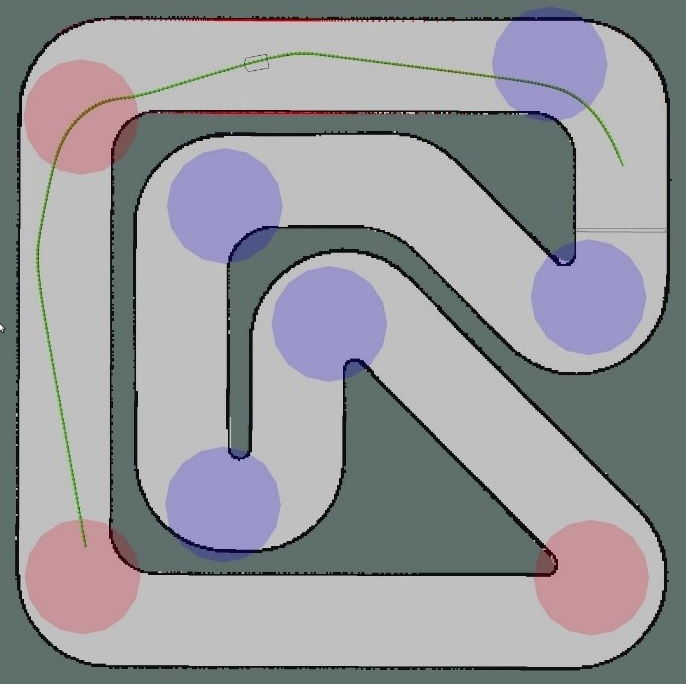
\includegraphics[width=0.5\textwidth]{../img/experiments/rviz-planned-track.jpg}
	\caption{This figure captures a planned trajectory and a vehicle on the testing track as it is shown in Rviz. The circles represent the positions of the corners detected by the track analysis algorithm. The circles marked in red are the next three corners ahead of the vehicle. The mostly green line represents the last planned trajectory. Green parts of the trajectory show where the vehicle is expected to drive fast and red parts would show where the vehicle should slow down.}
	\label{fig:rviz-planned-track}
\end{figure}

\paragraph{Reference Implementation}
The F1/10 Simulator repository contains a reference implementation of the Pure Pursuit algorithm which follows a fixed spline path divided sectors marked as “unrestricted”, “caution”, and “brake”, which tell the vehicle how to adjust its speed. We used this implementation as a baseline and we will compare our results against this implementation. This algorithm cannot react to any unexpected obstacles.

\paragraph{\gls{SEHS}/Hybrid A* and Pure Pursuit}
The first trajectory following algorithm we tested was the Pure Pursuit controller. We tested different values of the lookahead distance, and we settled on an adaptive look ahead distance linearly proportional to the speed of the vehicle. The lookahead was set to \SI{1.0}{\meter} for a stopped vehicle and \SI{1.5}{\meter} for the theoretical top speed. Lower lookahead distances caused the vehicle to oscillate and higher lookahead distances often resulted in the vehicle colliding with the apexes of the corners. This algorithm has no mechanism of avoiding unexpected obstacles which were not considered by the planning algorithm and pure pursuit would blindly hit an obstacle if the reference trajectory went through it.

\paragraph{\gls{SEHS}/Hybrid A* and \gls{DWA}}
The other controller we tested was the \gls{DWA} algorithm. This algorithm has several parameters which we tuned until we reached satisfying results. First parameter is the prediction horizon which determines for how long we predict the movement of the vehicle from the current measured state with a single examined action. Short prediction horizon does not give enough room to reveal differences between all the applicable actions and a long prediction horizon is unrealistic, because we change the action several times per second and it also eliminates many actions, because fixating one action for too long would likely lead to a collision. We achieved best results by setting the prediction horizon to \SI{0.6}{\second}.

The other parameters are the weights we assign to the error of the position of the vehicle, the error of its heading angle, the error of the speed of the vehicle, and the proximity to the obstacles ahead of the vehicle and nearby obstacles. In the end, the highest weight was assigned to the distance from obstacles and the second largest to the position error.

\paragraph{Results}

The reference implementation follows a predefined trajectory almost flawlessly and during a test run of 10 consecutive laps it reached an average lap time of \SI{26.410}{\second} with the top speed reaching \SI{4.08}{\meter\per\second} and the best lap time in this run was \SI{25.911}{\second}. For detailed statistics of lap times and speeds achieved by this algorithm, see Table~\ref{tbl:reference-impl}.

Our trajectory analysis algorithm correctly detects eight corners in the circuit. We set the planning algorithm to plan for the next 3 corners ahead of it. The planning time on the desktop computer ranged between \SI{100}{\milli\second} and \SI{300}{\milli\second} depending on the initial state and on the length and complexity of the circuit segment ahead of the vehicle.

The results of our simulated races can be found in Tables~\ref{tbl:dwa-sehs},~\ref{tbl:dwa-hybrid-astar},~\ref{tbl:pure-pursuit-sehs},~and~\ref{tbl:pure-pursuit-hybrid-astar}. The average lap times and the best lap times are shown in the following table:

\begin{figure}[h!]
	\centering
	\robustify\bfseries
	\begin{tabular}{c c S[detect-weight] S[detect-weight] S}
		\toprule
		Planning alg. & Following alg. & \text{Avg. lap time} & \text{Best lap time} & \text{Max. speed} \\
		 &  & [\si{\second}] & [\si{\second}] & [\si{\meter\per\second}]       \\
		\midrule
		SEHS & DWA & \bfseries 25.577 & \bfseries 23.815 & 4.04 \\
		Hybrid A* & DWA & 25.802 & 24.295 & 4.05 \\
		SEHS & Pure Pursuit & 27.168 & 25.850 & 4.03 \\
		Hybrid A* & Pure Pursuit & 27.484 & 25.667 & 4.01 \\
		\bottomrule
	\end{tabular}
\end{figure}

The SEHS algorithm produces trajectories which are more aggressive than the Hybrid A* algorithm. The trajectory is often very close to the boundary of the track. This results in faster lap times than the Hybrid A* counterpart. On the other hand, the SEHS-guided vehicle crashes into a wall more often than when the vehicle follows trajectories produced by Hybrid A*.

If we compare the results with the trajectories planned ahead of time for the whole track as shown in~\ref{fig:race_track}, especially the lap times of the first rounds when the vehicle starts from standstill, it is clear that the planning algorithm finds trajectories which the following algorithms cannot follow to the full extent. This is most likely due to the imperfections of the kinematic vehicle model. The vehicle cannot go through some of the corners at the planned speed without hitting the outer wall of the track and so it has to brake more. On the other hand, the planned trajectory is not too far off from the actual trajectory and it serves as a good guidance for the vehicle during the race.

\begin{table}
	\centering
	\begin{tabular}{c c c c c}
		\toprule
		& Lap time       & Traveled distance  & Average speed             & Maximum speed             \\
		& [\si{\second}] & [\si{\meter}]      & [\si{\meter\per\second}]  & [\si{\meter\per\second}]  \\
		\midrule
		1. & 27.876 & 84.72 & 3.25 & 4.06 \\
		2. & 26.208 & 87.07 & 3.37 & 4.08 \\
		3. & 26.381 & 86.91 & 3.38 & 4.07 \\
		4. & 26.279 & 86.75 & 3.36 & 4.06 \\
		5. & 26.484 & 87.00 & 3.35 & 4.05 \\
		6. & 26.172 & 86.96 & 3.37 & 4.07 \\
		7. & 26.366 & 87.03 & 3.37 & 4.07 \\
		8. & 26.227 & 86.54 & 3.37 & 4.08 \\
		9. & \textbf{25.911} & \textbf{85.83} & \textbf{3.37} & \textbf{4.05} \\
		10. & 26.199 & 86.39 & 3.36 & 4.06 \\
		\bottomrule
	\end{tabular}
	\caption{The results of ten consecutive laps achieved with the reference implementation of the Pure Pursuit algorithm following a predefined curve. This implementation was taken from the F1/10 Simulator GitHub repository.}
	\label{tbl:reference-impl}
\end{table}

\begin{table}
	\centering
	\begin{tabular}{c c c c c}
		\toprule
		    & Lap time       & Traveled distance  & Average speed             & Maximum speed             \\
		    & [\si{\second}] & [\si{\meter}]      & [\si{\meter\per\second}]  & [\si{\meter\per\second}]  \\
		\midrule
		1. & 28.915 & 83.79 & 3.19 & 3.97 \\
		2. & 25.953 & 88.10 & 3.43 & 3.94 \\
		3. & 25.671 & 90.88 & 3.50 & 4.01 \\
		4. & 24.872 & 85.40 & 3.44 & 4.01 \\
		5. & 25.851 & 86.18 & 3.35 & 4.02 \\
		6. & 25.880 & 89.87 & 3.47 & 4.02 \\
		7. & 25.102 & 86.75 & 3.47 & 4.04 \\
		8. & \bfseries 23.815 & 83.93 & 3.52 & 4.01 \\
		9. & 24.286 & 85.48 & 3.53 & 4.04 \\
		10. & 25.428 & 88.06 & 3.47 & 4.02 \\
		\bottomrule
	\end{tabular}
	\caption{The results of ten consecutive laps achieved with the combination of the SEHS and DWA algorithms in the Gazebo simulator.}
	\label{tbl:dwa-sehs}
\end{table}

\begin{table}
	\centering
	\begin{tabular}{c c c c c}
		\toprule
		& Lap time       & Traveled distance  & Average speed             & Maximum speed             \\
		& [\si{\second}] & [\si{\meter}]      & [\si{\meter\per\second}]  & [\si{\meter\per\second}]  \\
		\midrule
		1. & 29.746 & 85.88 & 3.17 &  3.94 \\
		2. & 25.096 & 87.10 & 3.53 &  4.01 \\
		3. & 24.478 & 83.99 & 3.43 &  4.05 \\
		4. & 25.569 & 86.33 & 3.39 &  3.92 \\
		5. & 25.503 & 86.49 & 3.39 &  3.80 \\
		6. & 27.935 & 89.02 & 3.35 &  3.92 \\
		7. & 25.404 & 86.69 & 3.42 &  3.82 \\
		8. & \bfseries 24.295 & 86.54 & 3.56 &  4.03 \\
		9. & 24.786 & 85.21 & 3.45 &  4.01 \\
		10. & 25.209 & 88.85 & 3.52 &  4.00 \\
		\bottomrule
	\end{tabular}
	\caption{The results of ten consecutive laps achieved with the combination of the Hybrid A* and DWA algorithms in the Gazebo simulator.}
	\label{tbl:dwa-hybrid-astar}
\end{table}

\begin{table}
	\centering
	\begin{tabular}{c c c c c}
		\toprule
		& Lap time & Traveled distance  & Average speed & Maximum speed             \\
		& [\si{\second}] & [\si{\meter}]      & [\si{\meter\per\second}]  & [\si{\meter\per\second}]  \\
		\midrule
		1. & 29.814 & 84.31 & 3.11 & 4.03 \\
		2. & \bfseries 25.850 & 85.62 & 3.32 & 4.02 \\
		3. & 26.012 & 87.41 & 3.38 & 4.01 \\
		4. & 26.325 & 87.24 & 3.32 & 4.00 \\
		5. & 26.845 & 87.69 & 3.28 & 3.95 \\
		6. & 28.549 & 90.89 & 3.25 & 4.00 \\
		7. & 26.863 & 88.27 & 3.30 & 4.00 \\
		8. & 26.520 & 86.62 & 3.29 & 3.95 \\
		9. & 26.663 & 87.56 & 3.30 & 4.00 \\
		10. & 28.242 & 90.68 & 3.29 & 4.00 \\
		\bottomrule
	\end{tabular}
	\caption{The results of ten consecutive laps achieved with the combination of the SEHS and Pure Pursuit algorithms in the Gazebo simulator. During the last lap, the vehicle hit a wall and was slowed down.}
	\label{tbl:pure-pursuit-sehs}
\end{table}

\begin{table}
	\centering
	\begin{tabular}{c c c c c}
		\toprule
		& Lap time & Traveled distance  & Average speed & Maximum speed             \\
		& [\si{\second}] & [\si{\meter}]      & [\si{\meter\per\second}]  & [\si{\meter\per\second}]  \\
		\midrule
		1. & 31.119 & 85.38 & 3.0 & 4.0 \\
		2. & 26.569 & 87.16 & 3.32 & 4.0 \\
		3. & 27.531 & 88.36 & 3.23 & 4.01 \\
		4. & 26.057 & 87.11 & 3.36 & 3.98 \\
		5. & 26.071 & 84.51 & 3.29 & 4.0 \\
		6. & 33.191 & 100.34 & 3.27 & 4.0 \\
		7. & 26.529 & 87.19 & 3.31 & 4.01 \\
		8. & 26.070 & 85.58 & 3.31 & 4.0 \\
		9. & \bfseries 25.667 & 86.18 & 3.35 & 3.99 \\
		10. & 26.039 & 85.07 & 3.29 & 4.0 \\
		\bottomrule
	\end{tabular}
	\caption{The results of ten consecutive laps achieved with the combination of the Hybrid A* and Pure Pursuit algorithms in the Gazebo simulator. The vehicle hit a wall during the 6-th lap and it got stuck for a brief moment.}
	\label{tbl:pure-pursuit-hybrid-astar}
\end{table}

Both the \gls{SEHS} and Hybrid A* algorithms proved to be fast enough and to produce good reference trajectories even for the vehicle as it was moving at its maximum speed in the simulator. The algorithms were able to produce new plans at a rate of up to \SI{10}{\hertz}. The only problem we were experiencing was a drop of the re-planning frequency in the middle section of the track. The algorithms were sometimes not able to find a trajectory in the series of a tight left run followed-up with a hairpin turn. Each of the trajectories the algorithm tested resulted in a collision with the boundary of the track. Most of the time, the car would slow down enough so that the algorithm could find a trajectory to the next waypoint, but sometimes the car would keep following the trajectory to its end and then it would not have anything to follow. The Pure Pursuit algorithm would immediately crash into the road boundary and get stuck. The \gls*{DWA} algorithm on the other hand can continue driving further just by prefering actions which keep the vehicle away from obstacles and road boundaries. Once the vehicle reaches the apex of the hairpin turn, the planning algorithm is able to find a collision-free trajectory to the waypoints ahead of the vehicle and it can continue the race with only a small impact on the lap time. The Hybrid A* algorithm performed slightly better in this regard and it was mostly the \gls*{SEHS} algorithm which occasionally failed to produce a trajectory. This seems to be in line with the issue the \gls*{SEHS} algorithm had with the complex ``Zurich'' circuit as shown in Figure~\ref{fig:zurich}.

Both the Pure Pursuit and the \gls*{DWA} algorithms worked well in the simulator after their parameters were tuned. The Pure Pursuit algorithm performed slightly worse than the reference implementation. The \gls*{DWA} algorithm on the other hand reached the fastest lap times of the three algorithms on average and it also managed to reach the fastest lap time of \SI{23.855}{\second}. On top of that, it was more robust thanks to the ability to continue driving forward even without a guiding trajectory and it is therefore the winner of this race.

\subsection{Obstacle Avoidance}

The vehicle detects the obstacles using the readings from the \gls*{LIDAR} scanner and using the Costmap ROS library. The obstacles are marked into the occupancy grid and the planning algorithms and the \gls*{DWA} following algorithm can account for these obstacles. The \gls*{DWA} algorithm filters out any actions which would likely lead to a collision if they were being applied during its lookahead period. For the remaining actions, it calculates the tracking error of the projected movement of the vehicle and the reference trajectory and the distance from any obstacle marked in the occupancy grid. It therefore prefers actions, which steer the vehicle away from any obstacles.

The Gazebo simulator allows us to place obstacles, such as cubes and cylinders, into the scene. We tried placing these obstacles in the path of the vehicle and we observed how the vehicle reacts to it. When the vehicle observes the obstacle from afar, it usually has no issue going around it, because the trajectory planning algorithm has enough time to account for the obstacle and go around it. During the next lap, the vehicle will already plan its way around the obstacle even when it is still around a corner or two. An example of the vehicle going around obstacles is shown in Figure~\ref{fig:obstacle-avoidance-gazebo} and Figure~\ref{fig:obstacle-avoidance-rviz}.

The most challenging scenario was several obstacles placed one after the other. The vehicle detects the first one but it hits the second one if the planned trajectory goes through the second obstacle. The vehicle often managed to mark the obstacle into the occupancy grid, but the DWA algorithm was often unable to avoid it. A second challenging scenario was a narrow passage between two obstacles. If the obstacles were not marked precisely, which was often the case, the track would either appear to be blocked to the vehicle or the passage as too narrow for the vehicle to align itself with it and fit inside. The planning algorithm would fail to find a trajectory through the passage. The vehicle would then run out of the planned reference trajectory and it would stop or crash into a wall.
\begin{figure}
	\centering
	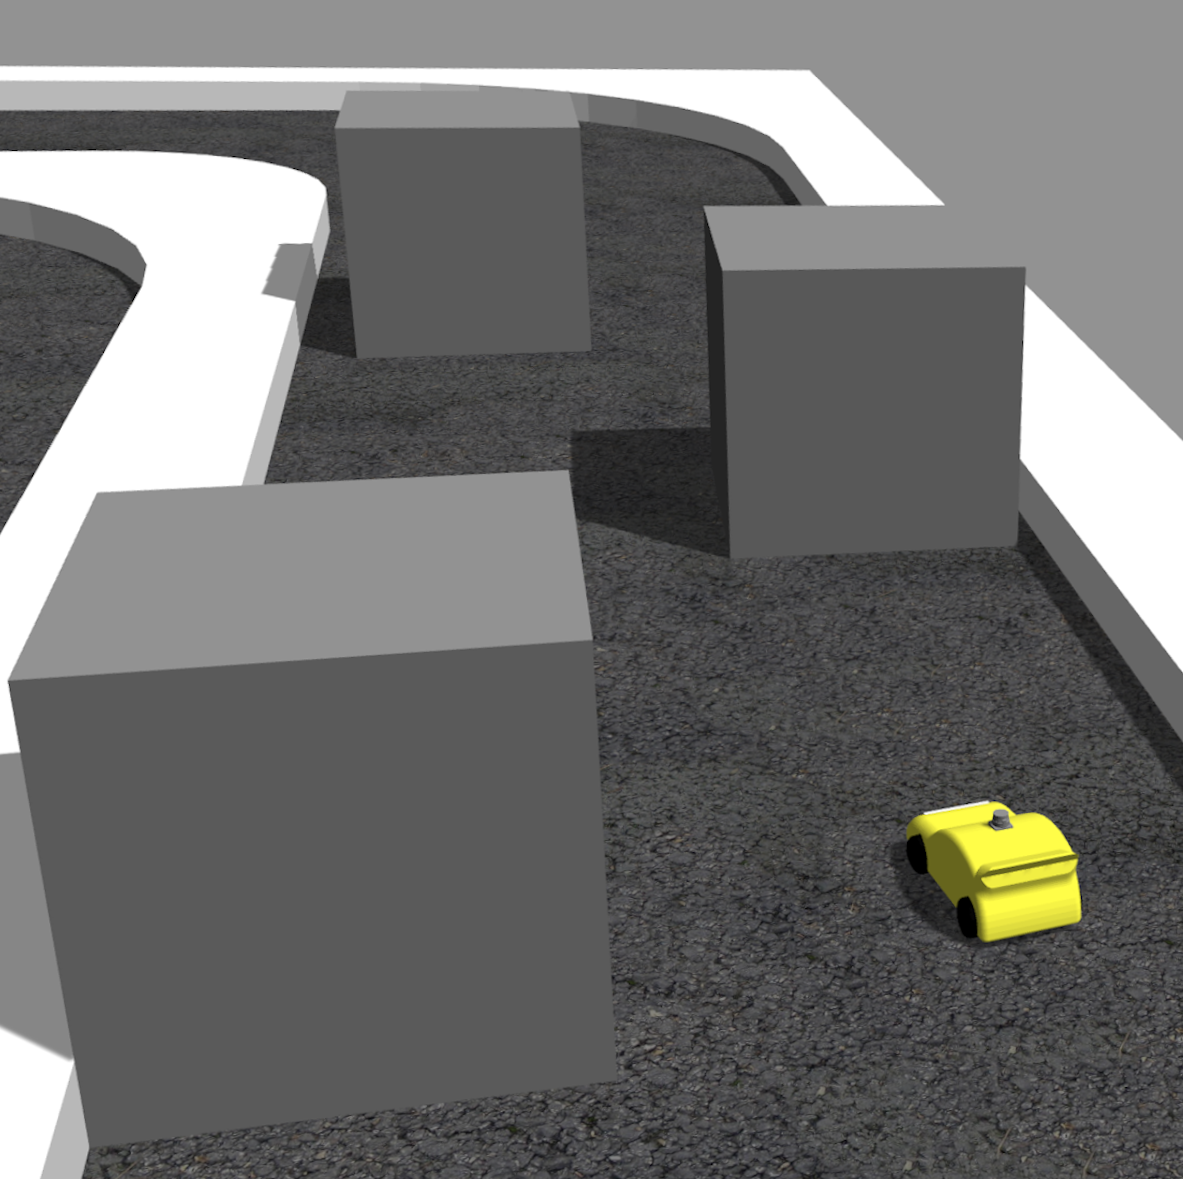
\includegraphics[width=\textwidth]{../img/experiments/simulator/obstacles-gazebo.png}
	\caption{The vehicle is passing three cubes in an alternating pattern.}
	\label{fig:obstacle-avoidance-gazebo}
\end{figure}

\begin{figure}
	\centering
	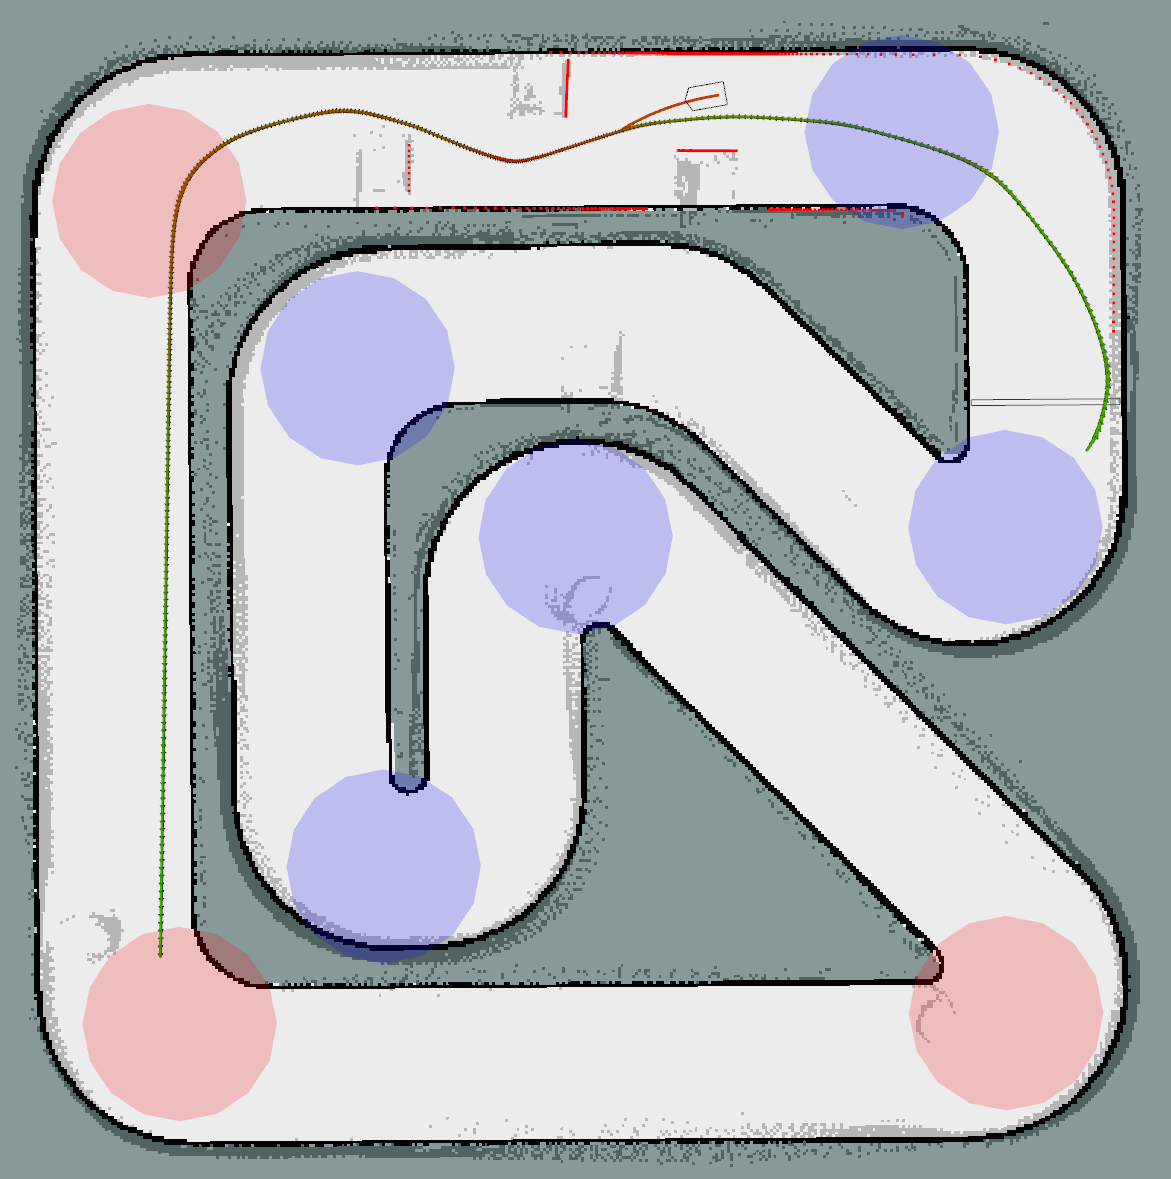
\includegraphics[width=\textwidth]{../img/experiments/simulator/obstacles-rviz.png}
	\caption{This picture shows how the information the vehicle has about its surroundings. The red dots are the readings from the LIDAR, black pixels show the original map of the track and the gray pixels are the detected obstacles which have been marked into the occupancy grid. The planned trajectory already accounted for the obstacles and it guides the vehicle through the narrow passage at a low speed.}
	\label{fig:obstacle-avoidance-rviz}
\end{figure}


